\documentclass[11pt,a4paper]{report}
\usepackage[textwidth=37em,vmargin=30mm]{geometry}
\usepackage{calc,xunicode,amsmath,amssymb,paralist,enumitem,tabu,booktabs,datetime2,xeCJK,xeCJKfntef,listings}
\usepackage{tocloft,fancyhdr,tcolorbox,xcolor,graphicx,eso-pic,xltxtra,xelatexemoji}

\newcommand{\envyear}[0]{2025}
\newcommand{\envdatestr}[0]{2025-10-21}
\newcommand{\envfinaldir}[0]{webdb/2025/20251021/final}

\usepackage[hidelinks]{hyperref}
\hypersetup{
    colorlinks=false,
    pdfpagemode=FullScreen,
    pdftitle={Web Digest - \envdatestr}
}

\setlength{\cftbeforechapskip}{10pt}
\renewcommand{\cftchapfont}{\rmfamily\bfseries\large\raggedright}
\setlength{\cftbeforesecskip}{2pt}
\renewcommand{\cftsecfont}{\sffamily\small\raggedright}

\setdefaultleftmargin{2em}{2em}{1em}{1em}{1em}{1em}

\usepackage{xeCJK,xeCJKfntef}
\xeCJKsetup{PunctStyle=plain,RubberPunctSkip=false,CJKglue=\strut\hskip 0pt plus 0.1em minus 0.05em,CJKecglue=\strut\hskip 0.22em plus 0.2em}
\XeTeXlinebreaklocale "zh"
\XeTeXlinebreakskip = 0pt


\setmainfont{Brygada 1918}
\setromanfont{Brygada 1918}
\setsansfont{IBM Plex Sans}
\setmonofont{JetBrains Mono NL}
\setCJKmainfont{Noto Serif CJK SC}
\setCJKromanfont{Noto Serif CJK SC}
\setCJKsansfont{Noto Sans CJK SC}
\setCJKmonofont{Noto Sans CJK SC}

\setlength{\parindent}{0pt}
\setlength{\parskip}{8pt}
\linespread{1.15}

\lstset{
	basicstyle=\ttfamily\footnotesize,
	numbersep=5pt,
	backgroundcolor=\color{black!5},
	showspaces=false,
	showstringspaces=false,
	showtabs=false,
	tabsize=2,
	captionpos=b,
	breaklines=true,
	breakatwhitespace=true,
	breakautoindent=true,
	linewidth=\textwidth
}






\newcommand{\coverpic}[2]{
    % argv: itemurl, authorname
    Cover photo by #2~~(\href{#1}{#1})
}
\newcommand{\makeheader}[0]{
    \begin{titlepage}
        % \newgeometry{hmargin=15mm,tmargin=21mm,bmargin=12mm}
        \begin{center}
            
            \rmfamily\scshape
            \fontspec{BaskervilleF}
            \fontspec{Old Standard}
            \fontsize{59pt}{70pt}\selectfont
            WEB\hfill DIGEST
            
            \vfill
            % \vskip 30pt
            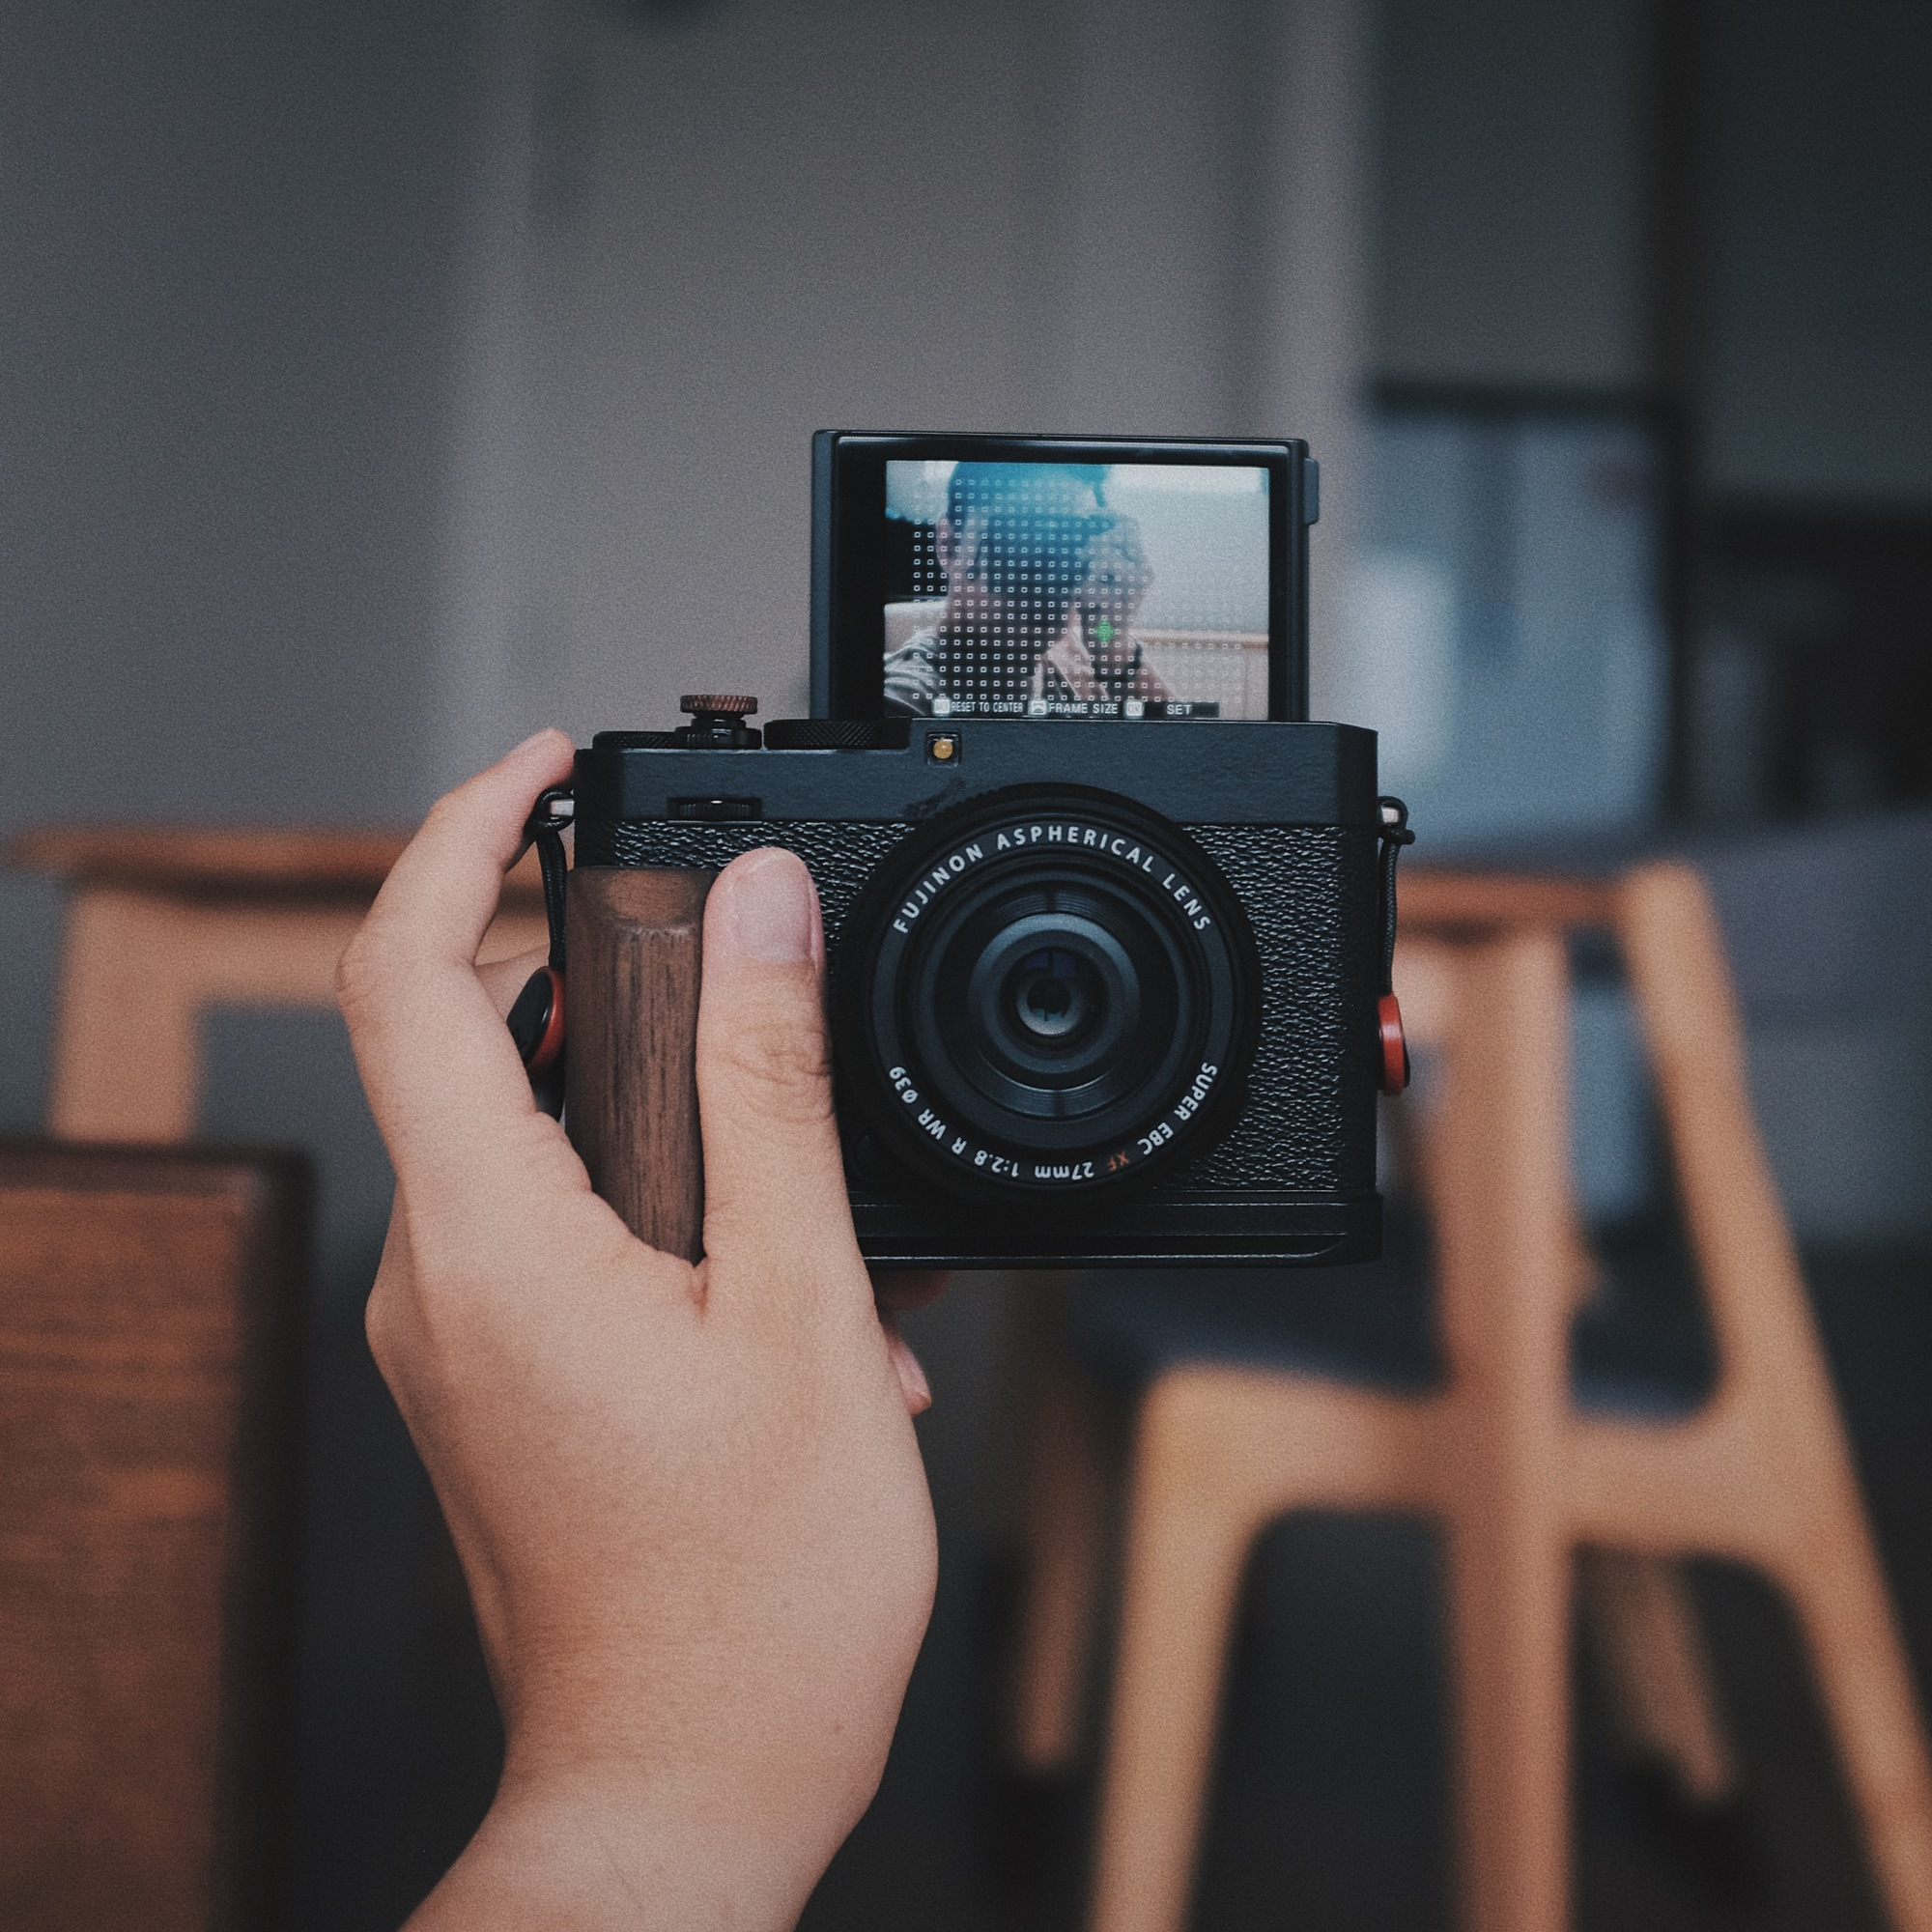
\includegraphics[width=\linewidth]{\envfinaldir/coverpic-prod.jpg}\par
            % \vskip 30pt
            \vfill

            \normalsize\rmfamily\scshape
            \copyright{} The Web Digest Project \hfill\large \envdatestr
        \end{center}
    \end{titlepage}
    % \restoregeometry
}
\newcommand{\simplehref}[1]{%
    \textcolor{blue!80!green}{\href{#1}{#1}}%
}
\renewcommand{\contentsname}{\center\Huge\sffamily\bfseries Contents\par\vskip 20pt}
\newcounter{ipartcounter}
\setcounter{ipartcounter}{0}
\newcommand{\ipart}[1]{
    % \vskip 20pt
    \clearpage
    \stepcounter{ipartcounter}
    \phantomsection
    \addcontentsline{toc}{chapter}{#1}
    % \begin{center}
    %     \Huge
    %     \sffamily\bfseries
    %     #1
    % \end{center}
    % \vskip 20pt plus 7pt
}
\newcounter{ichaptercounter}
\setcounter{ichaptercounter}{0}
\newcommand{\ichapter}[1]{
    % \vskip 20pt
    \clearpage
    \stepcounter{ichaptercounter}
    \phantomsection
    \addcontentsline{toc}{section}{\numberline{\arabic{ichaptercounter}}#1}
    \begin{center}
        \Huge
        \sffamily\bfseries
        #1
    \end{center}
    \vskip 20pt plus 7pt
}
\newcommand{\entrytitlefont}[1]{\subsection*{\raggedright\Large\sffamily\bfseries#1}}
\newcommand{\entryitemGeneric}[2]{
    % argv: title, url
    \parbox{\linewidth}{
        \entrytitlefont{#1}\par\vskip 5pt
        \footnotesize\ttfamily\mdseries
        \simplehref{#2}
    }\vskip 11pt plus 11pt minus 1pt
}
\newcommand{\entryitemGithub}[3]{
    % argv: title, url, desc
    \parbox{\linewidth}{
        \entrytitlefont{#1}\par\vskip 5pt
        \footnotesize\ttfamily\mdseries
        \simplehref{#2}\par\vskip 5pt
        \small\rmfamily\mdseries#3
    }\vskip 11pt plus 11pt minus 1pt
}
\newcommand{\entryitemAp}[3]{
    % argv: title, url, desc
    \parbox{\linewidth}{
        \entrytitlefont{#1}\par\vskip 5pt
        \footnotesize\ttfamily\mdseries
        \simplehref{#2}\par\vskip 5pt
        \small\rmfamily\mdseries#3
    }\vskip 11pt plus 11pt minus 1pt
}
\newcommand{\entryitemHackernews}[3]{
    % argv: title, hnurl, rawurl
    % \parbox{\linewidth}{
    %     \entrytitlefont{#1}\par\vskip 5pt
    %     \footnotesize\ttfamily\mdseries
    %     \simplehref{#3}\par
    %     \textcolor{black!50}{\href{#2}{#2}}
    % }\vskip 11pt plus 11pt minus 1pt
    \begin{minipage}{\linewidth}
            \entrytitlefont{#1}\par\vskip 5pt
            \footnotesize\ttfamily\mdseries
            \simplehref{#3}\par
            \textcolor{black!50}{\href{#2}{#2}}
    \end{minipage}\par\vskip 11pt plus 11pt minus 1pt
}







\begin{document}

\makeheader

\tableofcontents\clearpage




\ipart{Developers}
\ichapter{Hacker News}
\entryitemTwoLinks{Today is when the Amazon brain drain sent AWS down the spout}{https://news.ycombinator.com/item?id=45649178}{https://www.theregister.com/2025/10/20/aws\_outage\_amazon\_brain\_drain\_corey\_quinn/}

\entryitemTwoLinks{iOS 26.1 lets users control Liquid Glass transparency}{https://news.ycombinator.com/item?id=45648266}{https://www.macrumors.com/2025/10/20/ios-26-1-liquid-glass-toggle/}

\entryitemTwoLinks{J.P. Morgan's OpenAI loan is strange}{https://news.ycombinator.com/item?id=45648258}{https://marketunpack.com/j-p-morgans-openai-loan-is-strange/}

\entryitemTwoLinks{When a stadium adds AI to everything, it's worse experience for everyone}{https://news.ycombinator.com/item?id=45648249}{https://a.wholelottanothing.org/bmo-stadium-in-la-added-ai-to-everything-and-what-they-got-was-a-worse-experience-for-everyone/}

\entryitemTwoLinks{Claude Code on the web}{https://news.ycombinator.com/item?id=45647166}{https://www.anthropic.com/news/claude-code-on-the-web}

\entryitemTwoLinks{AWS outage shows internet users 'at mercy' of too few providers, experts say}{https://news.ycombinator.com/item?id=45646649}{https://www.theguardian.com/technology/2025/oct/20/amazon-web-services-aws-outage-hits-dozens-websites-apps}

\entryitemTwoLinks{Dutch spy services have restricted intelligence-sharing with the United States}{https://news.ycombinator.com/item?id=45646572}{https://intelnews.org/2025/10/20/01-3416/}

\entryitemTwoLinks{Chess grandmaster Daniel Naroditsky has died}{https://news.ycombinator.com/item?id=45646561}{https://old.reddit.com/r/chess/comments/1obnbmu/grandmaster\_daniel\_naroditsky\_has\_passed\_away/}

\entryitemTwoLinks{Production RAG: what I learned from processing 5M+ documents}{https://news.ycombinator.com/item?id=45645349}{https://blog.abdellatif.io/production-rag-processing-5m-documents}

\entryitemTwoLinks{Postman which I thought worked locally on my computer, is down}{https://news.ycombinator.com/item?id=45645172}{https://status.postman.com}

\entryitemTwoLinks{How much Anthropic and Cursor spend on Amazon Web Services}{https://news.ycombinator.com/item?id=45644777}{https://www.wheresyoured.at/costs/}

\entryitemTwoLinks{Commodore 64 Ultimate}{https://news.ycombinator.com/item?id=45644654}{https://www.commodore.net/product-page/commodore-64-ultimate-basic-beige-batch1}

\entryitemTwoLinks{BERT is just a single text diffusion step}{https://news.ycombinator.com/item?id=45644328}{https://nathan.rs/posts/roberta-diffusion/}

\entryitemTwoLinks{Servo v0.0.1}{https://news.ycombinator.com/item?id=45643357}{https://github.com/servo/servo}

\entryitemTwoLinks{Alibaba Cloud says it cut Nvidia AI GPU use by 82\% with new pooling system}{https://news.ycombinator.com/item?id=45643163}{https://www.tomshardware.com/tech-industry/semiconductors/alibaba-says-new-pooling-system-cut-nvidia-gpu-use-by-82-percent}

\entryitemTwoLinks{AI-generated 'poverty porn' fake images being used by aid agencies}{https://news.ycombinator.com/item?id=45643040}{https://www.theguardian.com/global-development/2025/oct/20/ai-generated-poverty-porn-fake-images-being-used-by-aid-agencies}

\entryitemTwoLinks{AWS Outage: A Single Cloud Region Shouldn't Take Down the World. But It Did}{https://news.ycombinator.com/item?id=45642951}{https://faun.dev/c/news/devopslinks/aws-outage-a-single-cloud-region-shouldnt-take-down-the-world-but-it-did/}

\entryitemTwoLinks{Matrix Conference 2025 Highlights}{https://news.ycombinator.com/item?id=45642923}{https://element.io/blog/the-matrix-conference-a-seminal-moment-for-matrix/}

\entryitemTwoLinks{Show HN: Playwright Skill for Claude Code – Less context than playwright-MCP}{https://news.ycombinator.com/item?id=45642911}{https://github.com/lackeyjb/playwright-skill}

\entryitemTwoLinks{Beaver-engineered dam in the Czech Republic}{https://news.ycombinator.com/item?id=45642562}{https://en.wikipedia.org/wiki/Beaver-engineered\_dam\_in\_the\_Czech\_Republic}\ichapter{Phoronix}
\entryitemGeneric{\hskip 0pt{}Patches Posted To Allow Hibernation Cancellation On Linux}{https://www.phoronix.com/news/Linux-Hibernation-Cancellation}

\entryitemGeneric{\hskip 0pt{}KosmicKrisp Vulkan To Apple Metal Driver Merged For Mesa 26.0}{https://www.phoronix.com/news/KosmicKrisp-Merged-Mesa-26.0}

\entryitemGeneric{\hskip 0pt{}AMD Announces "ROCm 7.9" As Technology Preview Paired With TheRock Build System}{https://www.phoronix.com/news/ROCm-Core-SDK-7.9}

\entryitemGeneric{\hskip 0pt{}AMD Ryzen 9 9950X vs. 9950X3D On Windows 11 \& Ubuntu Linux}{https://www.phoronix.com/review/windows-linux-amd-9950x-9950x3d}

\entryitemGeneric{\hskip 0pt{}Initial Tenstorrent Blackhole Support Aiming For Linux 6.19}{https://www.phoronix.com/news/Tenstorrent-Blackhole-Linux-619}

\entryitemGeneric{\hskip 0pt{}NTFSPLUS Announced: A New Linux Driver For NTFS With Better Performance, More Features}{https://www.phoronix.com/news/Linux-NTFSPLUS-NTFS-Driver}

\entryitemGeneric{\hskip 0pt{}Initial Intel Xe3P Graphics Support To Be Submitted For Linux 6.19}{https://www.phoronix.com/news/Intel-Xe3P-Starts-Linux-6.19}

\entryitemGeneric{\hskip 0pt{}Servo 0.0.1 Browser Engine Released}{https://www.phoronix.com/news/Servo-0.0.1-Released}

\entryitemGeneric{\hskip 0pt{}Linux 6.18-rc2 Released: "rc2 is on the bigger side"}{https://www.phoronix.com/news/Linux-6.18-rc2-Released}


\ipart{Developers~~~~(zh-Hans)}
\ichapter{Solidot}
\entryitemGeneric{\hskip 0pt{}AWS 宕机影响亚马逊和《堡垒之夜》等游戏}{https://www.solidot.org/story?sid=82588}

\entryitemGeneric{\hskip 0pt{}Xubuntu 官网被嵌入窃取加密货币的恶意程序}{https://www.solidot.org/story?sid=82587}

\entryitemGeneric{\hskip 0pt{}Windows 11 更新破坏了 Recovery Environment}{https://www.solidot.org/story?sid=82586}

\entryitemGeneric{\hskip 0pt{}日本电商巨头 ASKUL 遭勒索软件攻击}{https://www.solidot.org/story?sid=82585}

\entryitemGeneric{\hskip 0pt{}GIMP 正式提供 Snap 打包的版本}{https://www.solidot.org/story?sid=82584}

\entryitemGeneric{\hskip 0pt{}英伟达展示首块美制 Blackwell 芯片}{https://www.solidot.org/story?sid=82583}

\entryitemGeneric{\hskip 0pt{}7-Zip 远程代码执行漏洞 PoC 公开}{https://www.solidot.org/story?sid=82582}

\entryitemGeneric{\hskip 0pt{}GPT-5 并不能证明未解决的数学问题 }{https://www.solidot.org/story?sid=82581}

\entryitemGeneric{\hskip 0pt{}维基百科志愿者制服试图在大会上自杀的持枪男子}{https://www.solidot.org/story?sid=82580}

\entryitemGeneric{\hskip 0pt{}小鼠研究显示新疗法能在数小时内清除大脑中与痴呆症相关的斑块}{https://www.solidot.org/story?sid=82579}

\entryitemGeneric{\hskip 0pt{}物理学家杨振宁去世,享年 103 岁}{https://www.solidot.org/story?sid=82578}

\entryitemGeneric{\hskip 0pt{}维基百科称 AI 导致人类访问量下降}{https://www.solidot.org/story?sid=82577}\ichapter{V2EX}
\entryitemGeneric{\hskip 0pt{}[问与答] 想买台 miniLED 75 寸电视,有没好推荐的?}{https://www.v2ex.com/t/1167170}

\entryitemGeneric{\hskip 0pt{}[Amazon Web Services] AWS 重大故障!}{https://www.v2ex.com/t/1167169}

\entryitemGeneric{\hskip 0pt{}[iOS] iOS 26.1 Beta 4 增加「锁屏滑动打开相机」开关}{https://www.v2ex.com/t/1167168}

\entryitemGeneric{\hskip 0pt{}[问与答] 所谓看书,就是把要学的东西全部看完吗?}{https://www.v2ex.com/t/1167167}

\entryitemGeneric{\hskip 0pt{}[程序员] 好家伙, asana 崩了}{https://www.v2ex.com/t/1167166}

\entryitemGeneric{\hskip 0pt{}[分享发现] 一个不太一样的论坛,有兴趣可以玩玩儿~}{https://www.v2ex.com/t/1167165}

\entryitemGeneric{\hskip 0pt{}[Apple] 说个 macOS 26 的 Docker 液态玻璃的槽点}{https://www.v2ex.com/t/1167164}

\entryitemGeneric{\hskip 0pt{}[分享创造] 闲着无聊做了个 AI 改图工具-Nana banana}{https://www.v2ex.com/t/1167163}

\entryitemGeneric{\hskip 0pt{}[问与答] 前男友发疯,怎么断干净??}{https://www.v2ex.com/t/1167161}

\entryitemGeneric{\hskip 0pt{}[问与答] 最近的电信宽带一到晚上就特别卡}{https://www.v2ex.com/t/1167160}

\entryitemGeneric{\hskip 0pt{}[分享创造] DeepSeek OCR 已经可以测试效果了,看着没吹牛}{https://www.v2ex.com/t/1167158}

\entryitemGeneric{\hskip 0pt{}[问与答] 怎么给老年人维护抖音推荐喜好?}{https://www.v2ex.com/t/1167156}

\entryitemGeneric{\hskip 0pt{}[职场话题] 制造业信息技术岗位怎么样?}{https://www.v2ex.com/t/1167154}

\entryitemGeneric{\hskip 0pt{}[天黑以后] 20251020 午夜俱乐部}{https://www.v2ex.com/t/1167153}

\entryitemGeneric{\hskip 0pt{}[问与答] 请教有没有发现什么好的 磁力聚合搜索 的工具?}{https://www.v2ex.com/t/1167152}

\entryitemGeneric{\hskip 0pt{}[全球工单系统] 腾讯云崩了吗?}{https://www.v2ex.com/t/1167151}

\entryitemGeneric{\hskip 0pt{}[宽带症候群] 大家家里网络怎么架构的啊}{https://www.v2ex.com/t/1167150}

\entryitemGeneric{\hskip 0pt{}[加密货币] OKB 现在市值低,值得入。投资就是投团队。}{https://www.v2ex.com/t/1167149}

\entryitemGeneric{\hskip 0pt{}[分享发现] 一个可以部署在 cf worker 上面的 matrix chatgpt 机器人}{https://www.v2ex.com/t/1167148}

\entryitemGeneric{\hskip 0pt{}[职场话题] 大家面试带纸质的简历过去嘛?}{https://www.v2ex.com/t/1167147}

\entryitemGeneric{\hskip 0pt{}[Claude] 刚开始,还只是有奇怪的口癖,现在厉害了。。。}{https://www.v2ex.com/t/1167146}

\entryitemGeneric{\hskip 0pt{}[随想] 对电子产品有处女情节,一旦摔过或类似的情况,就感觉手机有内伤或者哪里多少有毛病}{https://www.v2ex.com/t/1167145}

\entryitemGeneric{\hskip 0pt{}[问与答] 请问今年双十一适合买电脑吗?}{https://www.v2ex.com/t/1167144}

\entryitemGeneric{\hskip 0pt{}[English] ``long time no see''}{https://www.v2ex.com/t/1167143}

\entryitemGeneric{\hskip 0pt{}[奇思妙想] 用 Manus 和 KIMI 做了一个 PIX 主题魔改教程小网站~~}{https://www.v2ex.com/t/1167139}

\entryitemGeneric{\hskip 0pt{}[问与答] 为什么中文网页链接喜欢在新窗口打开}{https://www.v2ex.com/t/1167138}

\entryitemGeneric{\hskip 0pt{}[写周报] 一人公司周记 02:门前竹影疏,后圃树荫棉}{https://www.v2ex.com/t/1167137}

\entryitemGeneric{\hskip 0pt{}[加密货币] 新的空投来了,撸起来}{https://www.v2ex.com/t/1167136}

\entryitemGeneric{\hskip 0pt{}[Apple] ios 知乎真是个坏 b 软件,只要屏蔽了广告就给你无限请求,狂消耗电量}{https://www.v2ex.com/t/1167133}

\entryitemGeneric{\hskip 0pt{}[Excel] JSON Excel Tool | Convert Excel, JSON, CSV \& More}{https://www.v2ex.com/t/1167131}

\entryitemGeneric{\hskip 0pt{}[分享发现] 能否不要再将 LLM 翻译成法学硕士,真的每次看到都会笑}{https://www.v2ex.com/t/1167130}

\entryitemGeneric{\hskip 0pt{}[生活] 世间还有吓人的犯罪恐怖惊悚片吗?}{https://www.v2ex.com/t/1167129}

\entryitemGeneric{\hskip 0pt{}[Apple] 好恶心..JD 广告上岛了?}{https://www.v2ex.com/t/1167128}

\entryitemGeneric{\hskip 0pt{}[Faucet] 乞讨,求 sol gas}{https://www.v2ex.com/t/1167126}

\entryitemGeneric{\hskip 0pt{}[分享创造] 做了一个 How Attractive am I 网站,中文是颜值打分}{https://www.v2ex.com/t/1167125}

\entryitemGeneric{\hskip 0pt{}[iPhone] iPhone air 未来将在中国大陆推出 eSIM 快速转换功能}{https://www.v2ex.com/t/1167124}

\entryitemGeneric{\hskip 0pt{}[VPS] 有没有办法给 vps 限制每月的总流量?}{https://www.v2ex.com/t/1167123}

\entryitemGeneric{\hskip 0pt{}[硬件] 网上买了一个硬件,连了一个摄像头,写了一些程序,怎么做好看的产品外观}{https://www.v2ex.com/t/1167122}

\entryitemGeneric{\hskip 0pt{}[问与答] 双十一来了,求便携屏推荐}{https://www.v2ex.com/t/1167121}

\entryitemGeneric{\hskip 0pt{}[分享创造] 做了个 YouTube 字幕批量下载工具,支持登录账号"批量"下载会员视频字幕}{https://www.v2ex.com/t/1167120}

\entryitemGeneric{\hskip 0pt{}[程序员] 基于 Java 手搓模块化的 MCP 服务器}{https://www.v2ex.com/t/1167119}

\entryitemGeneric{\hskip 0pt{}[酷工作] 深圳 wlb 小而美不内卷-小鹅通内推!}{https://www.v2ex.com/t/1167117}

\entryitemGeneric{\hskip 0pt{}[问与答] 请教使用多种 ai 工具的场景下,如何有效轮询检查任务状态?}{https://www.v2ex.com/t/1167115}

\entryitemGeneric{\hskip 0pt{}[酷工作] [深圳][腾讯会议、腾讯元宝] Android 研发工程师急招}{https://www.v2ex.com/t/1167114}

\entryitemGeneric{\hskip 0pt{}[信息安全] 前两天 ASP.NET Core 爆出来的 9.9 分超大漏洞 CVE-2025-55315 影响 ASP.NET Core 5.0/6.0 吗?}{https://www.v2ex.com/t/1167113}

\entryitemGeneric{\hskip 0pt{}[Solana] 每天优化一点点, 距离真正可用又前进了一小步}{https://www.v2ex.com/t/1167112}

\entryitemGeneric{\hskip 0pt{}[Google] Google 账户验证问题,求点帮助}{https://www.v2ex.com/t/1167109}

\entryitemGeneric{\hskip 0pt{}[程序员] 2025 年了, express 还在被 "DDOS"}{https://www.v2ex.com/t/1167108}

\entryitemGeneric{\hskip 0pt{}[职场话题] 京东社招流程就是狗屎}{https://www.v2ex.com/t/1167107}

\entryitemGeneric{\hskip 0pt{}[问与答] CORS 会被废除吗?}{https://www.v2ex.com/t/1167106}


\ipart{Generic News}







\clearpage
\leavevmode\vfill
\footnotesize

Copyright \copyright{} 2023-2025 Neruthes and other contributors.

This document is published with CC BY-NC-ND 4.0 license.

The entries listed in this newsletter may be copyrighted by their respective creators.

This newsletter is generated by the Web Digest project.

The newsletters are also delivered via Telegram channel \CJKunderline{\href{https://t.me/webdigestchannel}{https://t.me/webdigestchannel}}.\\
RSS feed is available at \CJKunderline{\href{https://webdigest.pages.dev/rss.xml}{https://webdigest.pages.dev/rss.xml}}.

This newsletter is available in PDF at
\CJKunderline{\href{https://webdigest.pages.dev/}{https://webdigest.pages.dev/}}.

The source code being used to generate this newsletter is available at\\
\CJKunderline{\href{https://github.com/neruthes/webdigest}{https://github.com/neruthes/webdigest}}.

This newsletter is also available in
\CJKunderline{\href{http://webdigest.pages.dev/readhtml/\envyear/WebDigest-20251021.html}{HTML}} and
\CJKunderline{\href{https://github.com/neruthes/webdigest/blob/master/markdown/\envyear/WebDigest-20251021.md}{Markdown}}.


\coverpic{https://unsplash.com/photos/beagle-dog-with-ears-flying-out-car-window-XSknXjyCVcs}{Hector O'Connor}


\end{document}
